\section{Noise Tunnel}

Noise Tunnel \cite{kokhlikyan2020captum} is not an attribution method but a technique that improves the accuracy of attribution methods. It combines SmoothGrad \cite{smilkov2017smoothgrad}, SmoothGrad-Square (unpublished version of the SmoothGrad), and VarGrad \cite{adebayo2018sanity} and works with most of the attribution methods.

\vspace{\baselineskip}

Noise Tunnel addresses a problem described in sections \ref{section:gbp} and \ref{section:ig}, where we discussed the problem with \textit{ReLU} activation function and gradients producing noisy, often irrelevant attributions. Because the partial derivative $\frac{\partial F_c}{\partial x_i}$ of the models' score $F_c$ for a class $c$ with respect to the value of the pixel $x_i$ fluctuates, Smilkov et al. \cite{smilkov2017smoothgrad} thought that adding a Gaussian noise ${\mathcal {N}}(0, 0.01^2)$ and calculating an average of sampled attributions is going to solve the problem.

\begin{equation}
\hat{M}_{c}(x)=\frac{1}{n} \sum_{1}^{n} M_{c}\left(x+\mathcal{N}\left(0, \sigma^{2}\right)\right)
\label{eq:smoothgrad}
\end{equation}

SmoothGrad (eq. \ref{eq:smoothgrad}) calculates the attribution ($M_c$) using any available method by providing that method an input with Gaussian noise. It then calculates a mean value from all the samples to reduce the importance of less frequent attributions. The idea is that when adding noise to the input image, important attributions are going to be visible most of the time, and noise might change between attributions.

\vspace{\baselineskip}

Another version of the SmoothGrad Noise Tunnel is SmoothGrad-Square. It changes only the way that the mean value is calculated by using the mean of squared attributions instead of just attributions (eq. \ref{eq:smoothgrad-sq}). This method usually provides less noisy results (compare Fig. \ref{fig:noisetunnel-smoothgrad-dingo} and Fig. \ref{fig:noisetunnel-smoothgrad-sq-dingo}) but often removes less important features, which are still valid features.

\begin{equation}
\hat{M}_{c}(x)=\frac{1}{n} \sum_{1}^{n} \sqrt{M_{c}\left(x+\mathcal{N}\left(0, \sigma^{2}\right)\right)}
\label{eq:smoothgrad-sq}
\end{equation}

The third version of Noise Tunnel is a version using VarGrad (see Fig. \ref{fig:noisetunnel-vargrad-dingo}) which is a variance version of the SmoothGrad and can be defined as Eq. \ref{eq:vargrad}, where $\hat{M}_c$ is a value of SmoothGrad. 

\begin{equation}
\tilde{M}_{c}(x)=\frac{1}{n} \sum_{k=1}^{n}\left\{M_{c}\left(x+\mathcal{N}\left(0, \sigma^{2}\right)\right)\right\}^{2}-\left\{\hat{M}_{c}(x)\right\}^{2}
\label{eq:vargrad}
\end{equation}

\begin{figure}[h]
  \centering
 \begin{subfigure}{.19\textwidth}
    \centering
    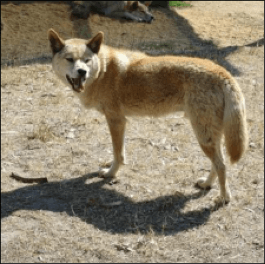
\includegraphics[width=\textwidth]{methods/images/dingo.png}
    \caption{Original image}\label{fig:noisetunnel-dingo}
\end{subfigure}
 \begin{subfigure}{.19\textwidth}
    \centering
    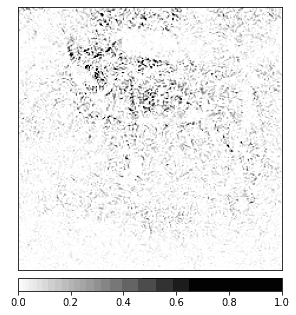
\includegraphics[width=\textwidth]{methods/images/ig-dingo.png}
    \caption{IG}\label{fig:noisetunnel-ig-dingo}
\end{subfigure}
 \begin{subfigure}{.19\textwidth}
    \centering
    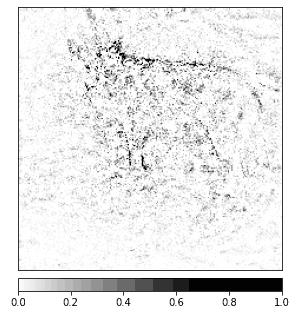
\includegraphics[width=\textwidth]{methods/images/ig-smoothgrad-dingo.png}
    \caption{SmoothGrad}\label{fig:noisetunnel-smoothgrad-dingo}
\end{subfigure}
 \begin{subfigure}{.19\textwidth}
    \centering
    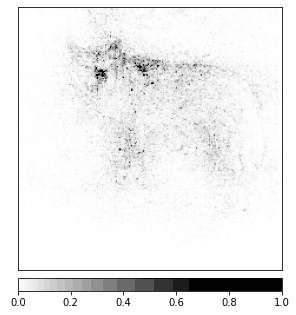
\includegraphics[width=\textwidth]{methods/images/ig-smoothgrad-sq-dingo.png}
    \caption{SmoothGrad-Sq}\label{fig:noisetunnel-smoothgrad-sq-dingo}
\end{subfigure}
 \begin{subfigure}{.19\textwidth}
    \centering
    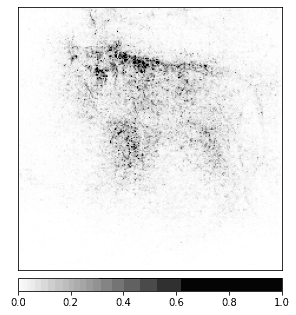
\includegraphics[width=\textwidth]{methods/images/ig-vargrad-dingo.png}
    \caption{VarGrad}\label{fig:noisetunnel-vargrad-dingo}
\end{subfigure}

 \caption{Visualisation of saliency maps produced by \textit{IG} (\ref{fig:noisetunnel-ig-dingo}), \textit{IG with SmoothGrad} (\ref{fig:noisetunnel-smoothgrad-dingo}), \textit{IG with SmoothGrad-Square} (\ref{fig:noisetunnel-smoothgrad-sq-dingo}), and \textit{IG with VarGrad} (\ref{fig:noisetunnel-vargrad-dingo}) of the same input image \ref{fig:noisetunnel-dingo} for a class \textit{dingo}. All the maps are generated using the same model (ResNet18). All noise tunnels are generating 10 random samples from ${\mathcal {N}}(0,1)$ distribution. Image source: \textit{Stanford Dogs} \cite{stanford-dogs} }\label{fig:noisetunnel-comparison-dingo}
\end{figure}

When comparing all the methods used in Noise Tunnel, we can see major differences in comparison with the original attribution (see Fig. \ref{fig:noisetunnel-comparison-dingo}). Using SmoothGrad (Fig. \ref{fig:noisetunnel-smoothgrad-dingo}) seams to detect more edges of the input image (in comparison with pure IG attribution in Fig. \ref{fig:noisetunnel-ig-dingo}), and that can be interpreted as detecting decision boundary. SmoothGrad-Square (Fig. \ref{fig:noisetunnel-smoothgrad-sq-dingo}) and VarGrad (Fig. \ref{fig:noisetunnel-vargrad-dingo}) are removing a large amount of noise but usually also some of the important features visible on the attribution from SmoothGrad (look on the tail of the dingo). In my work, if referring to Noise Tunnel, the default option will be the SmoothGrad version (unless specified otherwise).